\subsection{Attractive}
Es importante que la informacion resulte atractiva, llamativa, con chispa. No solo desde un punto de vista conceptual
o funcional como vimos en el apartado de relevante, donde dejamos claro la implicacion de los datos y la importancia
de su correcta presentacion, con una estructura que guie al usuario de una manera logica y ordenada.

Tiene que agarrar nuestra atencion, para ello podremos proponernos los siguientes requisitos, que sea divertida, entretenida,
moderna, actual, cercana, de calidad, bella y armonica.

Aunque estas caracteristicas sean subjetivas, existen tecnicas para poder lograr estos objetivos.

Otras caracteristicas mas tecnicas son:\\
 
\textbf{Consistencia.} Los controles que realizen las mismas acciones debe mantener el mismo diseno. Las funcionalidades
tambien deberan seguier este principio\\

\textbf{Limpieza.} Un diseno ordenado transmitira una mejor sensacion y el usuario sera capaz de localizar lo que busca
mas facilmente\\

\textbf{Simplicidad.} El objetivo es representar la informacion, huiremos de toda decoracion innecesaria que emborrene
el objetivo principal. Recordemos que menos es mas. Un diseno complicado, con muchos colores y diferentes formas abstractas
sera mas dificil de interpretar por el usuario\\


\textbf{Estandares.} En el mercado existen varios estandares a los que el usuario esta acostumbrado y sabe lo que esperar.
Por ejemplo una lupa, lo relacionamos con la accion de buscar, si utilizamos este icono, el usuario sabra rapidamente que
funcion realiza, sin embargo, si utilizamos uno completamente nuevo, puede incluso confundir al usuario\\

\textbf{Familiaridad.} Al usuario le resultara mas facil de manipular o navegar sobre la plataforma si siente que 
le es familiar y no se siente perdido. Por ejemplo, si tenemos un icono para elegir una fecha, seria muy recomendable
utilizar un calendario, aunque no es un estandar, estamos acostumbrados a reconocerlo\\

\textbf{Detalles.} Una etiqueta con distinta tipologia u otro color, puede disturbar a la percepcion del usuario. Si no 
buscamos resaltar algo en concreto, parecera un error \\

\textbf{Sena de identidad.} Es muy recomendable utilizar algo singular que nos identifique y que el usuario sea capaz 
de reconocernos rapidamente, esto puede ser una imagen, una combinacion de colores, un logo, etc.

\subsubsection{How to solve it} 
Para poder realizar un diseno atractivo, hay que estudiar las tendencias del momento, las buenas practicas de diseno y aplicarlas.
Es muy recomendable mantener un diseno simple y limpio, utilizar estandares u mecanismos que les resulten familiares a los usuarios,
cuidar los detalles y marcar nuestra identidad.


\subsubsection{How we solve it. Aire Guru} 
Como comentabamos anteriormente el diseno se ha basado en material design, utilizar lineas rectas, diferencia
distintas secciones mediante rectangulos y utiliza colores que constractan lo suficiente entre la informacion y el fondo.
El color de fondo para las graficas es el blanco, ya que la mayoria utilizan distintos colores y el blanco es un color 
neutro. Solo se utilza el tonalidades de azul, gris y blanco. Ademas se utiliza un tipo de letra facil de leer si decoracion.

Las secciones estan dispuestas ordenada y estructuradamente. Estas  se componen de una cabecera y un cuerpo. 

La pagina central se compone de una cabezera, el cuerpo y un pie de pagina. Tanto la cabecera y el pie de pagina son estaticos,
se muestran en todas las paginas y continen toda la informacion disponible para navegar entre paginas.
El cuerpo se divide en tres secciones horizontales, la zona superior con el mapa y la informacion general del punto seleccionado,
la zona media donde podemos filtrar los agentes contaminantes por condiciones medicas e informacion sobre la situacion actual y la 
zona inferior donde encontraremos el historial de zona y el personalizado.

\begin{figure}[ht]
    \centering
    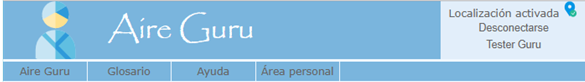
\includegraphics[width=12cm]{heading}
    \caption{Heading}
\end{figure}

Los componentes estandares son:
\begin{itemize}
 \item los botones, que se oscurecen cuando estan seleccionados y utilizar una tonalidad mas resultona cuando se seleccionan.
\item Pestanas, con un comportamiento similar y un aspecto de pestana estandar
\item Simbolo de espera, circulo rotatorio
\item Links, textos subrayados
\item Barra de busqueda, igual que la que encontramos en los buscadores
\end{itemize}



\begin{figure}[ht]
    \centering
   \subfigure[Searching bar]
    {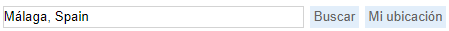
\includegraphics[width=5.5cm  ]{searchingBar}}
    \hfill
    \subfigure [Tabs]
       { 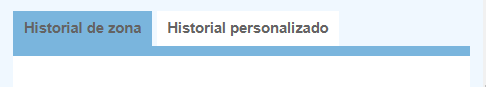
\includegraphics[width=5.5cm]{tabs}}
    \vfill
     \subfigure[Link]
     { \centering 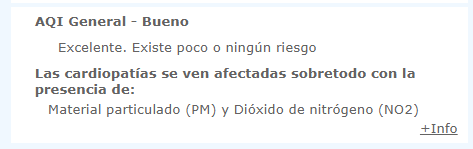
\includegraphics[width=6cm]{link}}
  
  \caption{Filters}
    \end{figure}
Los elementos que nos aportan familiaridad son la iconografia que utilizamos para mostrar el AQI. Utilizamos nubes, por representacion
del aire, el entorno, se acompana de un corazon si la calidad es buena, de un simbolo de exclamacion si es pobre, de una cruz si es 
mala y cambiamos a una mascara de gas si el estado es insalubre.

Hoy en dia todos estamos acostumbrados a los mapas de GoogleMaps, por ello se ha integrado para representar el mapa y no otro,
ya que los usuarios estan familiarizados por como se ven y en su manejo.

El simbolo de nuestra herramienta es un genio, es decir un guru, ademas, incluimos "Aire" en el logo, porque representa perfectamente
que mostramos. Nuestra herramienta es el genio del Aire.

Por ultimo, se ha tenido en cuenta que el usuario puede utilizar nuestra herramienta en distintos dispositivos, por lo que se han implementado 
dos formatos distintos, uno para pantallas mas amplias como el de ordenador y otro para formato mas pequeno para tableta o movil.


\elsparagraph{Evaluation}  
\begin{itemize}
    \done
    \crossed
    \crossed Aunque se han intentado implementar las lineas de diseno que estan ahora en el mercado, el diseno es mejorable
\end{itemize}

\newpage